\chapter{Results}
\label{chap:results}
The datasheet of our \ce{NdFeB} particles specifies that their residual magnetic field is \qtyrange{730}{760}{\milli\tesla}. Full saturation (\qty{>95}{\percent}) is achieved when a \qty{2}{\tesla} field is applied. Our method of magnetising the particle was limited to a \qty{1.4}{\tesla} field. As such, it is likely that we did not achieve the full saturation of the particle and that the residual magnetic field is lower than specified. Assuming a roughly linear relation between the two values, we estimate the residual magnetic field of our particles to be \qtyrange{510}{530}{\milli\tesla}. The density of the particles is given as \qty{7430}{\kilo\gram\per\cubic\meter}.

These values, together with the simulation of the magnetic field distribution in the trap, allows us to estimate the required driving frequency and the resulting eigen frequency.

\begin{figure}
    \centering
    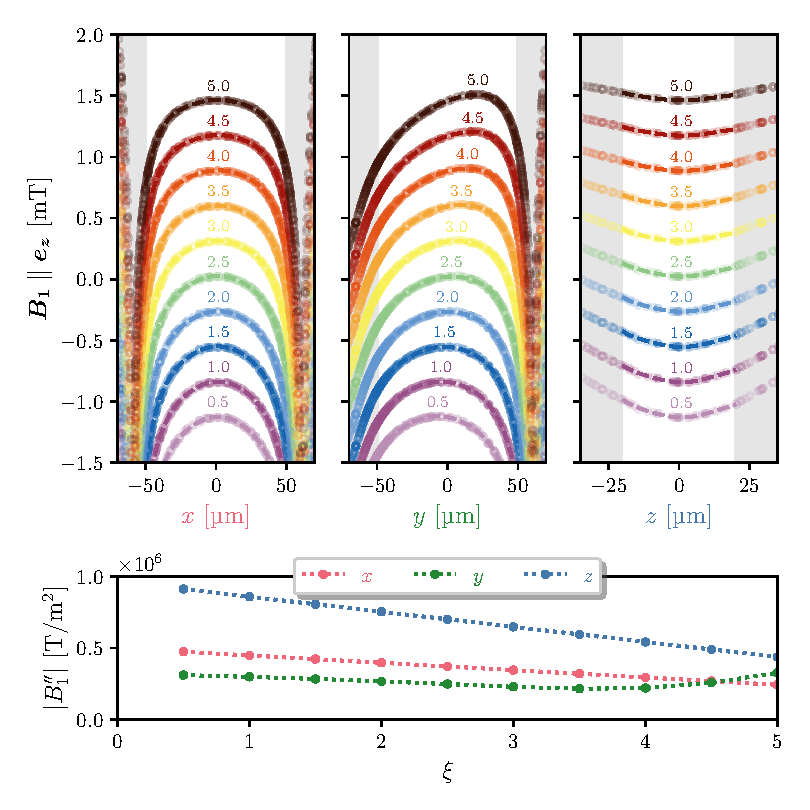
\includegraphics{figures/data/magnetic_field_curvature.pdf}
    \caption{the \textbf{top} figures from left to right show $z$-component of the magnetic field evaluated along a line parallel to the $x$-, $y$- and $z$-axis respectively through the origin. The gray zones indicate the boundaryies of the trap. The \textbf{bottom} figure shows the curvature of the magnetic field for these calculations evaluated in the extrema. The simulations were performed for $i_1=\qty{0.5}{\ampere}$ and $\chi$ between \numrange{-0.5}{-5}. The curves have been labelled with the corresponding value for $\chi$.}
    \label{fig:magnetic-field-curvature}
\end{figure}

\begin{figure}
    \centering
    \begin{subfigure}{0.5\textwidth}
        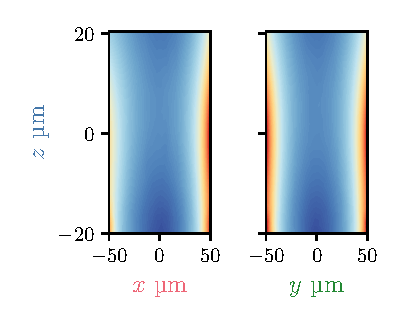
\includegraphics{figures/data/magnetic_field_distribution_in_trap_vertical.pdf}
    \end{subfigure}%
    \begin{subfigure}{0.5\textwidth}
        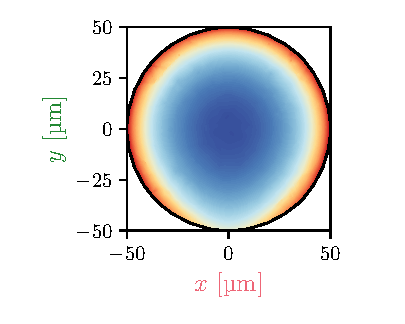
\includegraphics{figures/data/magnetic_field_distribution_in_trap_horizontal.pdf}
    \end{subfigure}
    \caption{The magnitude of $\vec{B_1} \parallel \zhat$ in the trap for $i_1=\qty{0.5}{\ampere}$ and $\chi=2$. The \textbf{left} (\textbf{right}) figure shows the magnetic field distribution in the vertical planes (horizontal plane). Towards the edges of the trap (nearer to the tracks) the magnetic field is stronger.}
    \label{fig:magnetic-field-distribution}
\end{figure}

\begin{figure}
    \centering
    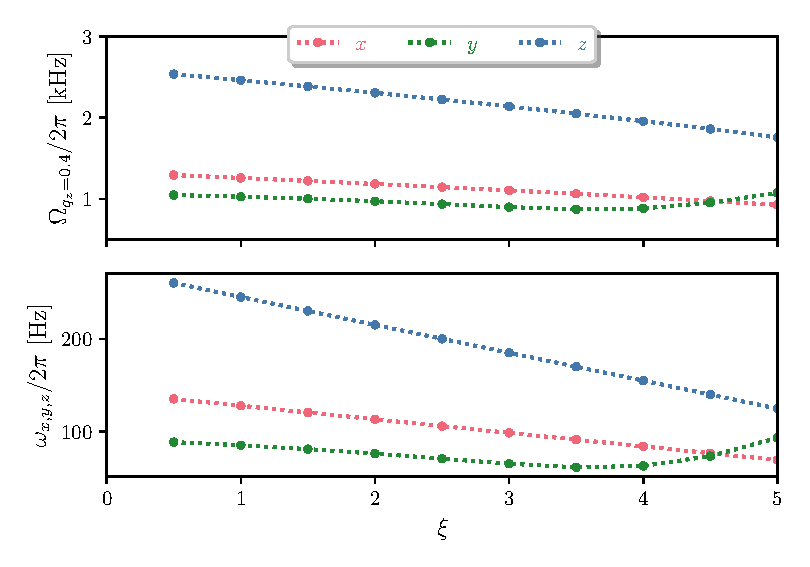
\includegraphics{figures/data/eigen_frequency_xi_dependence.pdf}
    \caption{Simulation results of the dependence of the eigen frequency on $\chi$. These results are based on the data presented in \autoref{fig:magnetic-field-curvature}. The \textbf{top} figure shows the minimal trapping frequency such that $q_z \leq 0.4$. In the \textbf{middle} the corresponding eigenfrequencies of the modes are shown for $\Omega / 2\pi = \qty{2.5}{\kilo\hertz}$. The \textbf{bottom} figure shows the deviation from the center of the \ymode. This is due the fact that the slit is in the direction of the \ymode. The dashed lines are a linear interpolation of the data and only serve as a guide to the eyes.}
\end{figure}

\section{Measurements at atmospheric pressure}
\label{sec:measurements-at-atmospheric-pressure}
TODO: change this to only mention the x-mode? As we did not drive the y-mode separately.
At atmospheric pressure we determined the dependence of $\omega_{x,y}$ on $\Omega$ and $i_1$. In these measurements the ratio $\xi$ was kept constant. The spectra are obtained using the lock-in amplifier connected to the photodiode. Due to the low Q-factor at atmospheric pressure, it is not possible to tell the $x$- and $y$-modes apart. The results are shown in \autoref{fig:xy-mode-dependence-1bar}. The $z$-mode is not visible in these measurements. In addition to this the dependence of the rotational mode on $B_0$ is shown in \autoref{fig:rotational-mode-dependence-1bar}. We note three curves with a apparently linear dependence on $B_0$. The two additional curves are modulations of the resonance peak with the trapping frequency. A fourth curve can be seen in the bottom right. Its origin is unclear. A fit has not been made due to the sparsity of the data. $\omega_\alpha$ has not been observed.

\begin{figure}
    \centering
    \begin{subfigure}{0.5\textwidth}
        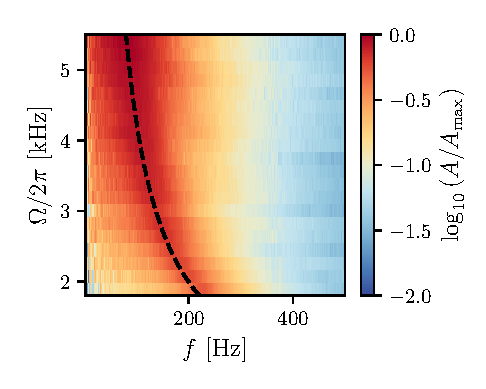
\includegraphics{figures/data/xy_mode_dependence_on_driving_frequency.pdf}
        %\label{fig:xy-mode-dependence-on-driving-frequency-1bar}
    \end{subfigure}%
    \begin{subfigure}{0.5\textwidth}
        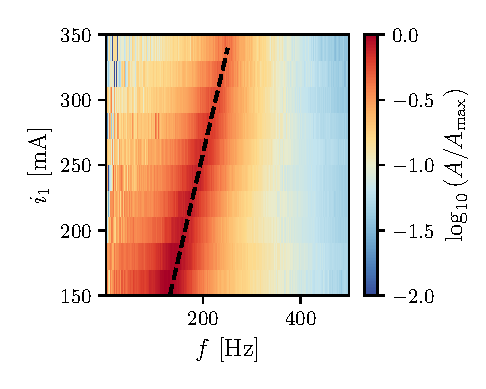
\includegraphics{figures/data/xy_mode_dependence_on_inner_current.pdf}
        %\label{fig:xy-mode-dependence-on-inner-current-1bar}
    \end{subfigure}
    \caption{The dependence of $\omega_{x,y}$ on $\Omega$ (\textbf{left}) and $i_1$ (\textbf{right}) at atmospheric pressure. The dashed lines are a fit following the theory of $\omega_{x,y}(\Omega) \sim 1 / \Omega$ and $\omega_{x,y}(i_1) \sim i_1$. The corresponding prefactors are $2\pi \cdot \qty{377.33170211685874\pm9.030914540546724}{\kilo\hertz\per\hertz}$ and \qty{626.5282946695123\pm20.984120764687987}{\hertz\per\ampere}. The normal value for $\Omega = 2\pi \cdot \qty{2.5}{\kilo\hertz}$ and $i_1 = \qty{200}{\milli\ampere}$ when they are not part of the sweep, the ratio $\chi = 2$ is always kept constant.}
    \label{fig:xy-mode-dependence-1bar}
\end{figure}

\begin{SCfigure}
    \centering
    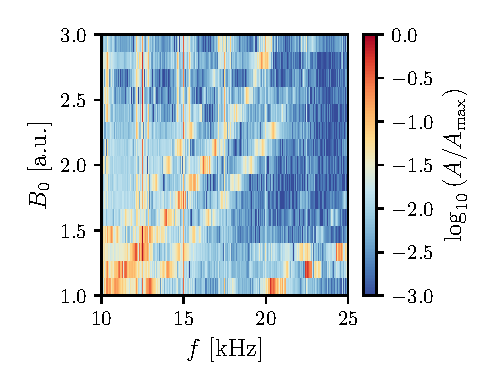
\includegraphics{figures/data/rotational_mode_dependence_on_B0.pdf}
    \caption{The dependence of $\omega_{\gamma,\tilde\beta}$ on $B_0$ at atmospheric pressure.}
    \label{fig:rotational-mode-dependence-1bar}
\end{SCfigure}

\section{Measurements at low pressure}
\label{sec:measurements-at-low-pressure}
At \qty{1}{\milli\bar} the readout was performed using the Thorcam and analysed using our custom object tracking algorithm. The reason to no longer use laser readout is due to the heating of the particle. By equating the power of the laser to Stefan-Boltzmann law we find that, in equillibrium assuming no heat dissipation through air, the temperature of the particle could reach \qty{2500}{\kelvin}. Even if only a fraction of the laser power would reach the particle this would be enough to reach its Curie temperature. Lower laser powers lead to an insufficient signal-to-noise ratio. We will return to this in the discussion.

\begin{SCfigure}
    \centering
    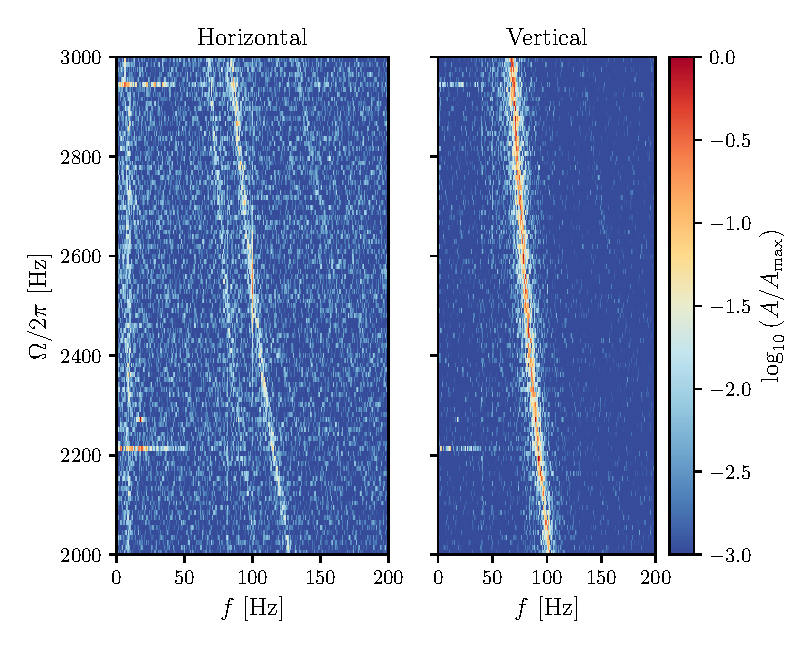
\includegraphics{figures/data/xyz_mode_dependence_on_driving_frequency_spectrum.pdf}
    \caption{The dependence of $\omega_{x,y,z}$ on $\Omega$ at \qty{1}{\milli\bar}. Shown are two directions (horizontal and vertical), they live in the $xy$-plane but do not directly match to the \xmode / \ymode, a small rotation angle needs to be taken into account.}
    \label{fig:xyz-mode-dependence-1mbar}
\end{SCfigure}

\autoref{fig:xyz-mode-dependence-1mbar} shows the dependence of $\omega_{x,y,z}$ at \qty{1}{\milli\bar}. We note that compared to the measurements at atmospheric pressures that the width of the peak is significantly smaller. Whilst this measurement shows a clear dependence of $\omega_{x,y,z}$ on $\Omega$, it is very difficult to see the \zmode. These measurements were obtained by continiously sweeping the driving frequency. Instead, we can do a `lock-in like' measurement. Here we set a fixed driving frequency and take a single spectrum before changing the driving frequency again. In the analysis we can simply match look at the peaks matching with the driving frequency. Thus making a `lock-in like' measurement. An example of such a measurement is shown in \autoref{fig:xyz-mode-spectrum-1mbar}.

\begin{SCfigure}
    \centering
    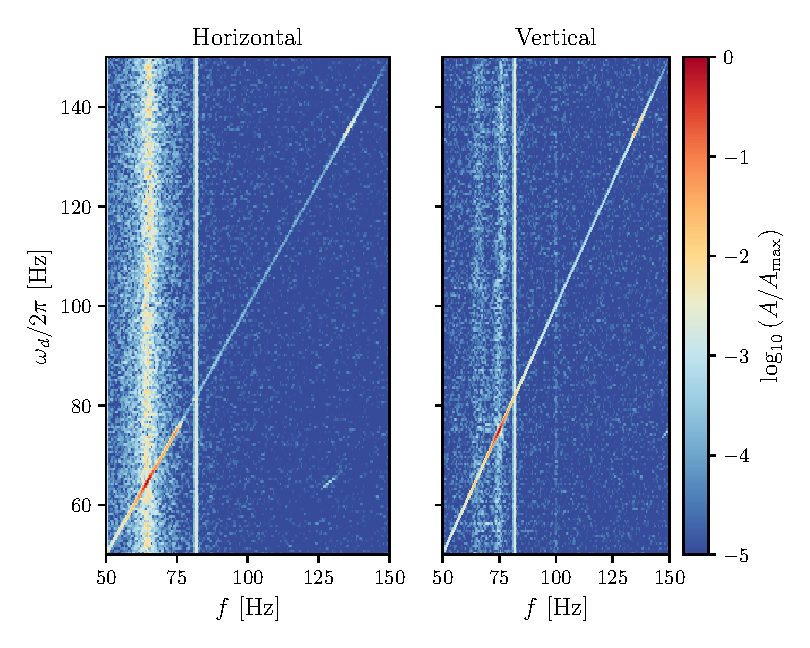
\includegraphics{figures/data/xyz_mode_spectrum.pdf}
    \caption{A PSD with a visible \xmode, \ymode and \zmode. The diagonal line is caused by the changing driving frequency. By looking at the magnitude along the diagonal line the eigenfrequencies and Q-factors can be }
    \label{fig:xyz-mode-spectrum-1mbar}
\end{SCfigure}

By performing this `lock-in like' measurement at multiple driving frequencies we can determine clear relations between $\omega_{x,y,z}$, the damping and the driving frequency. We do so by fitting a Lorentzian for each peak in the spectrum. The results are shown in \autoref{fig:xyz-mode-dependence-on-trapping-frequency-1mbar}. The fits are given by:
\begin{align}
    \omega_x &= \frac{\qty{ 11.394193305319426 \pm 0.6168138640026458 }{\square\kilo\hertz}}{\Omega} + (\qty{ -130.8583313665632 \pm 35.52389434927459 }{\hertz}) \\
    \omega_y &= \frac{\qty{ 8.61031330605224 \pm 0.3506111962572132 }{\square\kilo\hertz}}{\Omega} + (\qty{ -47.01583771770941 \pm 21.39358314176167 }{\hertz}) \\
    \omega_z &= \frac{\qty{ 19.211603271753344 \pm 0.9219280210953733 }{\square\kilo\hertz}}{\Omega} + (\qty{ -142.4727024226977 \pm 53.88080820095942 }{\hertz})
\end{align}

\begin{figure}
    \centering
    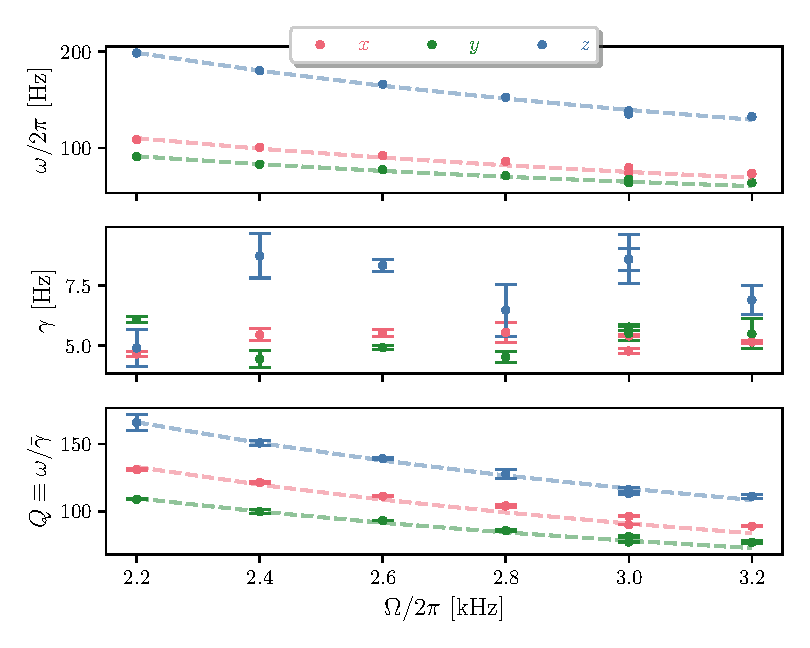
\includegraphics{figures/data/xyz_mode_dependence_on_driving_frequency.pdf}
    \caption{The dependence of $\omega_{x,y,z}$ and $\gamma_{x,y,z}$ on $\Omega$ at \qty{1}{\milli\bar}. The $\gamma$ in this case is the width of the Lorentzian fitted on the PSD. The dashed lines are a fit.}
    \label{fig:xyz-mode-dependence-on-trapping-frequency-1mbar}
\end{figure}

Visually it appears that $\gamma$ is constant as a function of $\Omega$. The question is whether $\gamma_z$ differs significantly from $\gamma_{x,y}$. To test this we perform a $T$-test on the mean values, the results can be found in \autoref{tab:gamma-t-test}. From this we can conclude that $\gamma_x = \gamma_y$ and $\gamma_z \gg \gamma_{x,y}$ at \qty{1}{\milli\bar}.

\begin{SCtable}
    \centering
    \begin{tabular}{cc}
        \toprule
        $H_0$ & $p$ \\
        \midrule
        $\gamma_x = \gamma_y$ & \textcolor{x_axis_color}{$0.897 \gg 0.05$} \\
        $\gamma_y = \gamma_z$ & \textcolor{y_axis_color}{$0.005 \ll 0.05$} \\
        $\gamma_x = \gamma_z$ & \textcolor{y_axis_color}{$0.005 \ll 0.05$} \\
        % $\gamma_x, \gamma_y \leq \gamma_z$ & \num{0.003} \\
        \bottomrule
    \end{tabular}
    \caption{The results of the $T$-test on the mean values of $\gamma_{x,y,z}$ from the data in \autoref{fig:xyz-mode-dependence-on-trapping-frequency-1mbar}.}
    \label{tab:gamma-t-test}
\end{SCtable}



\section{Q-factor dependence on pressure}
\label{sec:q-factor-dependence-on-pressure}
Using an external coil we are able to excite the \xmode  and \ymode seperately. Ringdown measurements are performed to determine the pressure dependence on the Q-factor. The Q-factor in this case is defined as $Q = \omega_{x,y} \cdot \tau / 2$ where $\tau$ is the decay time of the oscillation ($\sim \exp\left(t / \tau\right)$). We qualitatively observed a strong dependence of the Q-factor on the driving amplitude. When the driving amplitude is too high we observe non-linear time dependent behaviour. The results in \autoref{fig:q-factor-pressure-dependence} are obtained with a sufficiently low driving amplitude.

\begin{figure}
    \centering
    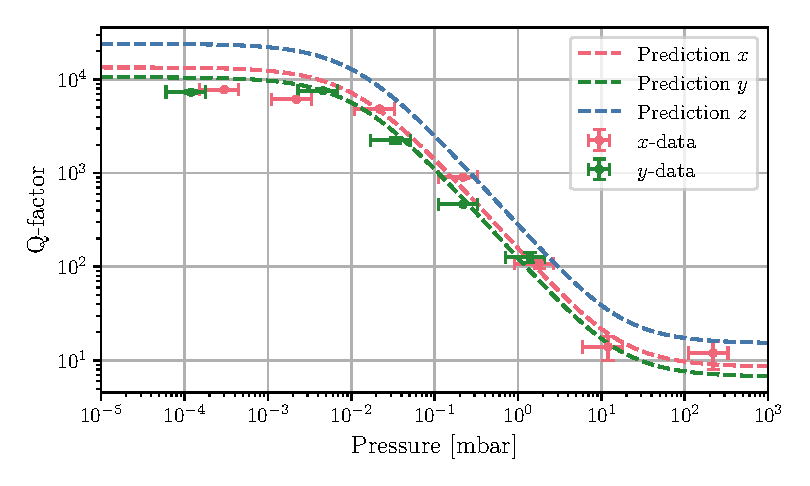
\includegraphics{figures/data/q_factor_pressure_dependence.pdf}
    \caption{The pressure dependence of the Q-factor for the $x$-, $y$- and $z$-mode. The dashed lines are a prediction based on the theory from \autoref{subsec:q-factor}. The experimental Q-factors are determined using the ringdown method. The \zmode has not been observed experimentally. The \xmode and \ymode were driven sinusoidally at their respective resonance frequencies.}
    \label{fig:q-factor-pressure-dependence}
\end{figure}
